\DiaryEntry{Exponential Distribution with Uniform parameter (Incomplete Gamma Functions)}{2019-06-01}{Stochastic}

We consider a random variable $X$ with exponential distribution,

\bee
f_X(x) = a e^{-ax}, \quad x \geq 0
\eee

In addition, the parameter $a$ is not considered constant but also a random variable with uniform distribution; 

\bee
f_a(a) = \begin{cases} 1 & \quad A \leq a \leq B \\ 0 & \quad \text{otherwise} \end{cases}
\eee

In this case, the pdf of $X$ given a certain value of $a$ is still exponential; i.e.

\bee
f(X|a) = a e^{-ax}, \quad x \geq 0
\eee

The pdf of $X$ is then this $f(X|a)$ averaged across the values of $a$: 

\bee
f_X(x) = \int_a f(X|a) f(a) da = \int_{a=A}^B a e^{-ax} da = \cdots = \frac{(Ax+1)e^{-Ax} - (Bx+1)e^{-Bx}}{x^2}
\eee

where Maxima helped a bit. Note that this is no longer an exponential distribution, but "something else". The Figure below shows the histogram of $X$ (blue) together with the histograms of an exponential distribution with $a=1$ (red) and $a=2$ (green). The histogram is in between the histograms of the two exponential distribution; a fact which intuitively makes sense as the uniform disitrubtion of the parameter $a$ averages the two exponential distributions.


\begin{figure}[hbt!]
\centering
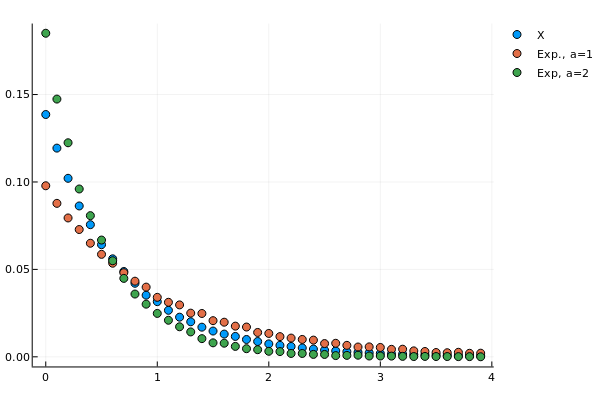
\includegraphics[scale=0.7]{images/exp_rv_uniform_param_01.png}
\end{figure}

We can use this pdf like a normal one; e.g. to calculate $P(X > b)$:

\bee
P(X > L) = \int_L^\infty f_X(x)dx = \int_L^\infty \frac{(Ax+1)e^{-Ax} - (Bx+1)e^{-Bx}}{x^2} dx
\eee

The resulting integral above is a bit tricky and involves the incomplete Gamma function.

The Gamma function (see also \ref{2015-07-27:entry}) itself is defined according to

\bee
\Gamma(x) = \int_0^\infty t^{x-1}e^{-t} dt
\eee

The extension with a general lower limit is the \emph{upper incomplete Gamma function} $\Gamma(s,x)$ 

\bee
\Gamma(s,x) = \int_x^\infty t^{s-1} e^{-t} dt
\eee

Rewriting above integrals a bit yields 

\bee
P(X > L) = \int_L^\infty Ax^{-1}e^{-Ax} + x^{-2} e^{-Ax} dx - \int_L^\infty Bx^{-1}e^{-Bx} + x^{-2} e^{-Bx} dx
\eee

Considering the first integral, we substitute $u = Ax \rightarrow x^{-1} = Au^{-1}, x^{-2} = A^2 x^{-2}$, $\frac{du}{dx} = A$, and $\frac{dx}{du} = 1/A$ and obtain

\bee
\int_L^\infty Ax^{-1}e^{-Ax} + x^{-2} e^{-Ax} dx = \int_{LA}^\infty A^2 u^{-1}e^{-u} + A^2 u^{-2} e^{-u} \frac{du}{A} = A \Gamma(0, LA) + A \Gamma(-1, LA)
\eee

Note that the integral limit have also changed due to the substitution. Therefore the probability becomes

\bee
P(X > L) = A \Gamma(0, LA) + A \Gamma(-1, LA) - B \Gamma(0, LB) - B \Gamma(-1, LB)
\eee

Note: It seems to be rather tricky to evaluate the incomplete Gamma function (e.g. in Julia); one way is to use the cdf of a Gamma distribution, but (at least in Julia), negative values for $s$ are not supported.

What is also interesting is to reparametrize the pdf $f(a)$ to e.g.

\bee
\tilde{f}(X|a) = a^2 e^{-a^2 x}, \quad x \geq 0
\eee

This will not change the pdf $f_X(x)$ and the whole reparametrization can be treated as integral substitution with $a = u^2, da = 2u du$,

\begin{align*}
f_X(x) = \int_a f(X|a) f(a) da &= \int_{a=A}^B a e^{-ax} da = \int_{u=\sqrt{A}}^{\sqrt{B}} u^2 e^{-u^2 x} 2u du \\ &= \int_{u=\sqrt{A}}^{\sqrt{B}} 2 u^3 e^{-u^2 x} du = \int_{u=\sqrt{A}}^{\sqrt{B}} 2 u u^2 e^{-u^2 x} du = \int_{u=\sqrt{A}}^{\sqrt{B}} \tilde{f}(u) \tilde{f}(X|u) du
\end{align*}

from which follows that the distribution of $u$, $\tilde{f}(u)$ is

\bee
\tilde{f}(u) = \begin{cases} 2u & \quad \sqrt{A} \leq a \leq \sqrt{B} \\ 0 & \quad \text{otherwise} \end{cases}
\eee



%%% Local Variables:
%%% mode: latex
%%% TeX-master: "journal"
%%% End:
